\documentclass[11pt,a4paper]{article}
\usepackage[utf8]{inputenc}
\usepackage[T1]{fontenc}
\usepackage{amsmath}
\usepackage[margin=2.5cm]{geometry}
\usepackage{booktabs}
\usepackage{graphicx}
\usepackage{caption}
\usepackage{hyperref}
\usepackage{tikz}
\usepackage{listings}
\usepackage{xcolor}
\usetikzlibrary{shapes.geometric, arrows.meta, positioning}
\usepackage{float}

\renewcommand{\figurename}{Figura}
\renewcommand{\tablename}{Tabla}
\renewcommand{\refname}{Referencias}
\renewcommand{\abstractname}{Resumen}

\lstset{
  basicstyle=\ttfamily\small,
  breaklines=true,
  frame=single,
  numbers=none,
  columns=fullflexible,
  backgroundcolor=\color{gray!8}
}

\hypersetup{
    colorlinks=true,
    linkcolor=black,
    citecolor=black,
    urlcolor=blue,
    pdftitle={TA-IND-02 - Analisis de Consistencia y Replicacion en BDD Distribuidas},
}

\title{\textbf{TA-IND-02 --- Informe Técnico Individual}\\
\large Análisis de Consistencia y Replicación en BDD Distribuidas}
\author{
Estudiante: Keyla Betzabe Bedón Viteri \\
Equipo PFC: BCEL -- SGA Escuela de Educación Básica Provincias Unidas \\
Microservicio a cargo del autor: Docente \\
Docente: Ing. Guerrero Ulloa Gleiston Cicero, PhD \\
Asignatura: Aplicaciones Distribuidas (ISR-701) \\
Unidad 3 -- Bases de Datos Distribuidas \\
Período académico: 2026--2027
}
\date{14 de julio de 2026}

\begin{document}

\maketitle

\begin{abstract}
\noindent
Este informe analiza el modelo de consistencia y replicación adoptado por el microservicio Docente dentro del Proyecto de Fin de Curso (PFC) del equipo BCEL, un Sistema de Gestión Académica (SGA) para la Escuela de Educación Básica Provincias Unidas, organizado en microservicios independientes (Principal/Autenticación, Secretaría, Docente, Soporte técnico).
A diferencia de un esquema de base de datos compartida, el equipo BCEL adoptó el patrón \emph{database-per-service}: el microservicio Principal opera sobre su propia instancia PostgreSQL (Spring Boot) y el microservicio Docente opera sobre una instancia PostgreSQL independiente en Supabase (Django REST Framework), comunicándose mediante REST y gRPC, con réplicas de lectura configuradas sobre la base del microservicio Docente. Este informe caracteriza dicho modelo a la luz del espectro de consistencia y de los marcos CAP y PACELC, argumentando que la ausencia de claves foráneas físicas entre servicios traslada la integridad referencial a llamadas RPC síncronas contra el microservicio Principal, mientras que la replicación asíncrona de lectura introduce un riesgo concreto de \emph{staleness} en los reportes académicos (boletas, promedios) que el microservicio genera. Se evalúan dos alternativas replicación síncrona y desacoplamiento mediante caché local con eventos frente al modelo vigente, concluyendo que este último es razonable para la fase académica del PFC pero requiere mitigaciones concretas antes de un despliegue con tráfico real.
\end{abstract}

\section{Introducción}

El PFC del equipo BCEL implementa el Sistema de Gestión Académica (SGA) de la Escuela de Educación Básica Provincias Unidas, organizado en microservicios independientes que se comunican mediante un microservicio Principal que actúa como gateway de autenticación y de comunicación inter-servicio. El autor de este informe es responsable del microservicio
\textbf{Docente}, construido sobre Django y Django REST Framework, cuya base de datos PostgreSQL reside en una instancia gestionada de Supabase bajo el esquema \texttt{sga\_docente}.

El microservicio Docente administra nueve módulos de negocio: Actividades, Calificaciones, Asistencias, Resumen de asistencia, Promedios trimestrales, Promedios anuales, Detalle de promedios anuales, Seguimiento académico y Períodos de evaluación. Estos módulos concentran la lógica de evaluación del estudiante incluida la fórmula de promedio trimestral
(\(\text{promedio\_trimestral} = \text{promedio\_formativo} \times 0.70 + \text{nota\_sumativa}
\times 0.30\)), el cálculo del promedio anual y la conversión de notas cuantitativas a la escala cualitativa institucional (DAR, AAR, PAR, NAR) por lo que la corrección e integridad de sus datos tiene impacto directo sobre documentos oficiales del estudiante, como la boleta trimestral y el concentrado de calificaciones.

A diferencia del caso analizado en otros equipos del curso, en los que varios microservicios
comparten una única instancia de base de datos separada únicamente por esquemas, el equipo BCEL decidió que cada microservicio posea su propia instancia física de base de datos: el microservicio Principal opera sobre PostgreSQL propio (Spring Boot) y el microservicio
Docente opera sobre una instancia PostgreSQL independiente (Django, Supabase), comunicándose
mediante REST y gRPC. Además, sobre la base de datos del microservicio Docente se han configurado réplicas de lectura. Esta combinación \emph{database-per-service} más replicación de lectura ocupa una posición particular dentro del espectro de consistencia que este informe caracteriza con precisión.

El presente informe responde a la pregunta orientadora de la unidad: \textbf{¿es el modelo de consistencia elegido el óptimo para el dominio del sistema?} El objetivo es caracterizar formalmente el modelo \emph{database-per-service} con réplicas de lectura implementado para el microservicio Docente, contrastarlo con al menos dos alternativas documentadas en la literatura, y sostener una postura razonada sobre su optimalidad, sus riesgos y las mitigaciones aplicables.

\section{Marco Teórico}

\subsection{El espectro de modelos de consistencia}

La consistencia en sistemas de almacenamiento distribuido no es una propiedad binaria, sino
un espectro ordenado por la fuerza de las garantías que ofrece a los clientes de las réplicas
\cite{viotti2016}. En un extremo se ubica la linealizabilidad (o consistencia fuerte), que
exige que toda operación parezca ejecutarse de forma instantánea en un punto entre su invocación y su reconocimiento, de modo que todas las réplicas perciban un único orden total compatible con el tiempo real \cite{viotti2016}. Le sigue la consistencia secuencial, que exige un orden total acordado por todos los clientes pero relaja la restricción de tiempo real, y la consistencia causal, que solo exige preservar el orden entre operaciones causalmente relacionadas. Particularmente relevante para el caso del microservicio Docente es la garantía de \emph{lectura de los propios cambios} (read-your-writes), una de las garantías centradas en el cliente que Viotti y Vukolić distinguen de las garantías centradas en los datos: un docente que acaba de registrar una calificación espera que, al generar inmediatamente después un reporte, esa calificación ya esté reflejada \cite{viotti2016}. En el
extremo más débil se encuentra la consistencia ventual, que únicamente garantiza que, en ausencia de nuevas escrituras, todas las réplicas convergerán al mismo valor. Bailis y Ghodsi remarcan que, en la práctica, la consistencia eventual y sus variantes son adoptadas por
compromisos concretos de latencia y disponibilidad, y que la elección entre un modelo más fuerte o más débil debe hacerse considerando explícitamente esos compromisos, tal como los describen CAP y PACELC \cite{bailis2013}.

\subsection{Teoremas de compromiso: CAP y PACELC}

El teorema CAP, formalizado por Gilbert y Lynch a partir de la conjetura original de Brewer, establece que ante una partición de red un sistema distribuido no puede garantizar simultáneamente consistencia y disponibilidad; debe sacrificar una de las dos mientras la partición persiste \cite{gilbert2002}. Abadi observó que esta lectura es incompleta, dado que CAP solo describe el comportamiento del sistema durante una partición, un evento poco frecuente en la mayoría de los despliegues; propuso entonces la formulación PACELC: en presencia de una Partición (P), el sistema elige entre Availability (A) y Consistencia (C); pero \emph{Else} (E), en operación normal sin particiones, el sistema elige entre Latencia (L) y Consistencia
(C) \cite{abadi2012}. Una revisión reciente sobre el diseño integral de sistemas de bases de datos distribuidas remarca que este compromiso debe leerse de forma continua a lo largo de todo el ciclo de vida del sistema, y no como una decisión puntual de arquitectura
\cite{carvalho2025}.

\subsection{Estrategias de replicación}

La estrategia de replicación determina qué nivel de consistencia es alcanzable en la práctica.
En la replicación primario-respaldo (\emph{leader-follower}), un único nodo líder acepta todas
las escrituras y las propaga a uno o más nodos seguidores; si la propagación es síncrona, el
sistema puede sostener consistencia fuerte a costa de mayor latencia de escritura, mientras que si es asíncrona se introduce un retraso de replicación (\emph{staleness} acotado) a cambio de menor latencia de escritura y mayor disponibilidad de lectura \cite{bailis2013}. Los sistemas de referencia industrial ilustran los extremos de este espectro: Dynamo, el almacén
clave-valor de Amazon, prioriza explícitamente la disponibilidad mediante replicación sin líder por quorum y consistencia eventual con resolución de conflictos del lado del cliente \cite{decandia2007}; en el extremo opuesto, Spanner ofrece consistencia externa apoyándose en TrueTime, un servicio de sincronización de relojes con incertidumbre acotada \cite{corbett2013}.

\subsection{El patrón \emph{database-per-service} y la integridad referencial entre microservicios}

Laigner, Zhou y Vaz Salles argumentan que el patrón \emph{database-per-service}, si bien favorece el aislamiento de fallos a nivel de microservicio, traslada una carga sustancial de gestión de datos hacia la capa de aplicación, obligando a los equipos de desarrollo a resolver manualmente problemas de integridad referencial y consistencia entre servicios que antes resolvía el motor de base de datos de forma nativa \cite{laigner2021}. Kanwal et al. muestran
que, al eliminarse las restricciones de clave foránea nativas entre los límites de los microservicios, la integridad referencial debe sostenerse mediante mecanismos alternativos validación por API síncrona, comunicación orientada a eventos, o el patrón Saga con transacciones compensatorias cada uno con distintos compromisos entre consistencia, disponibilidad y complejidad operativa \cite{kanwal2025}. Shabani et al. complementan esta discusión desde una perspectiva arquitectónica más general, mostrando que la descomposición de
un sistema monolítico en microservicios introduce ganancias de escalabilidad y mantenibilidad, pero a costa de mayor complejidad de coordinación entre los componentes distribuidos
\cite{shabani2021}.

\section{Análisis del Modelo de Consistencia del PFC}

\subsection{Caracterización del modelo implementado}

El equipo BCEL adoptó, para el microservicio Docente, el patrón \emph{database-per-service} en su forma más estricta: el microservicio Principal (Spring Boot) opera sobre su propia instancia PostgreSQL, y el microservicio Docente (Django REST Framework) opera sobre una instancia PostgreSQL físicamente independiente, alojada en Supabase bajo el esquema \texttt{sga\_docente}. No existe una base de datos compartida entre servicios ni claves foráneas físicas que crucen de una instancia a otra. Sobre la instancia del microservicio Docente se ha configurado, además, al menos una réplica de lectura.

La Figura~\ref{fig:topologia} ilustra la topología: dos instancias PostgreSQL físicamente independientes una por microservicio, comunicadas mediante REST/gRPC, con una réplica de lectura desprendida de la instancia primaria del microservicio Docente.

\begin{figure}[H]
\centering
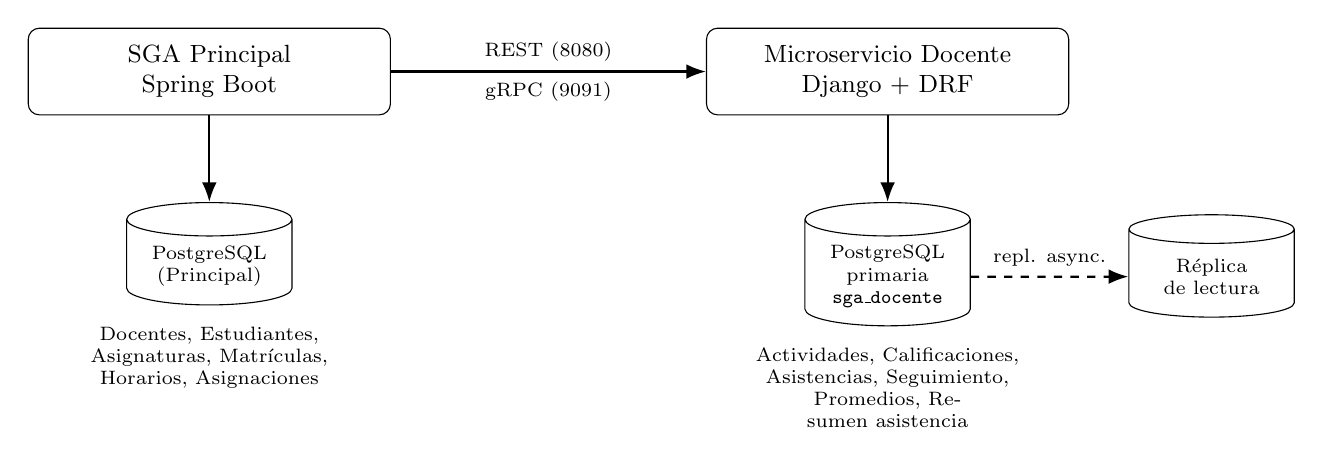
\begin{tikzpicture}[
    node distance=1.1cm and 1.6cm,
    box/.style={rectangle, draw, rounded corners, minimum width=4.6cm, minimum height=1.1cm, align=center, font=\small},
    db/.style={cylinder, draw, shape border rotate=90, aspect=0.25, minimum height=1.3cm, minimum width=2.1cm, align=center, font=\scriptsize},
    arr/.style={-{Latex[length=2.5mm]}, thick}
]

\node[box] (principal) {SGA Principal\\Spring Boot};
\node[db, below=of principal] (dbprincipal) {PostgreSQL\\(Principal)};
\node[below=0.15cm of dbprincipal, font=\scriptsize, align=center, text width=3.4cm] (modprincipal)
  {Docentes, Estudiantes,\\Asignaturas, Matrículas,\\Horarios, Asignaciones};

\node[box, right=4.0cm of principal] (docente) {Microservicio Docente\\Django + DRF};
\node[db, below=of docente] (dbdocente) {PostgreSQL\\primaria\\\texttt{sga\_docente}};
\node[db, right=2cm of dbdocente] (replica) {Réplica\\de lectura};
\node[below=0.15cm of dbdocente, font=\scriptsize, align=center, text width=3.6cm] (moddocente)
  {Actividades, Calificaciones,\\Asistencias, Seguimiento,\\Promedios, Resumen asistencia};

\draw[arr] (principal) -- (dbprincipal);
\draw[arr] (docente) -- (dbdocente);
\draw[arr, dashed] (dbdocente) -- node[above, font=\scriptsize]{repl. async.} (replica);

\draw[arr] (principal.east) -- node[above, font=\scriptsize]{REST (8080)} node[below, font=\scriptsize]{gRPC (9091)} (docente.west);

\end{tikzpicture}
\caption{Topología del modelo de datos del microservicio Docente dentro del PFC de BCEL: dos instancias PostgreSQL físicamente independientes (patrón \emph{database-per-service}), comunicadas por REST/gRPC, con una réplica de lectura sobre la instancia primaria del microservicio Docente. No existen claves foráneas físicas entre las dos bases de datos.}
\label{fig:topologia}
\end{figure}

Esta separación de instancias tiene un correlato exacto en la propiedad de los datos. El microservicio Principal administra las entidades de \emph{catálogo} y de \emph{matrícula} del sistema: Docentes, Estudiantes, Asignaturas, Matrículas, Horarios y Asignaciones, mientras que el microservicio Docente administra únicamente las entidades de \emph{evaluación} generadas durante el período lectivo: Actividades, Calificaciones, Asistencias, Seguimiento académico, Promedios y Resumen de asistencia. 

En consecuencia, todo identificador que el microservicio Docente recibe y persiste como referencia a un estudiante, una asignatura o una asignación docente-materia (\texttt{id\_matricula}, \texttt{id\_asignacion}) apunta a un registro cuya fuente de verdad reside físicamente en la base de datos del microservicio Principal, y no en el esquema \texttt{sga\_docente}.

Esta correspondencia exacta entre módulos y microservicios es la que hace concreto, y no solo teórico, el problema de integridad referencial entre servicios descrito por Kanwal et al. y Laigner et al. para el patrón \emph{database-per-service}: no existe ni puede existir, al tratarse de instancias físicamente separadas una clave foránea física de \texttt{calificaciones.id\_matricula} hacia \texttt{matriculas.id} en el sentido en que la definiría un motor relacional dentro de una misma base de datos. 

La comunicación entre servicios sigue dos caminos complementarios. Primero, el frontend del microservicio Docente nunca invoca gRPC directamente: toda solicitud pasa por el microservicio Principal, que actúa como \emph{gateway} (REST en el puerto 8080 hacia el frontend, gRPC en el puerto 9091 hacia Docente para las consultas que el Principal necesita resolver). Segundo, y en
sentido inverso, el propio microservicio Docente valida el contexto y los permisos del docente autenticado llamando de vuelta al microservicio Principal mediante un servicio gRPC dedicado (\texttt{TeacherContextService}, expuesto en el puerto 9092). Esta segunda ruta es la que resuelve, en tiempo de escritura, la integridad referencial que en un esquema compartido resolvería una clave foránea: cuando el microservicio Docente registra una calificación o una
asistencia asociada a un \texttt{id\_matricula} o a un \texttt{id\_asignacion}, esos identificadores no existen físicamente en el esquema \texttt{sga\_docente}; son referencias lógicas a entidades cuya fuente de verdad reside en otro microservicio, y su validez se confirma o se asume válida sin una llamada explícita adicional en el momento de la solicitud HTTP/gRPC, no mediante una restricción del motor de base de datos.

El Listado~\ref{lst:endpoint} muestra uno de los \emph{endpoints} de negocio del microservicio Docente cuyo cálculo depende enteramente de datos que residen en su propia instancia, pero cuya validez de entrada (identidad del estudiante y de la asignación) depende de una fuente externa.

\begin{lstlisting}[caption={Endpoint de cálculo de promedio trimestral del microservicio Docente.}, label={lst:endpoint}]
POST /api/docente/promedios-trimestrales/calcular/
Content-Type: application/json

{
  "id_matricula": 1,
  "id_asignacion": 10,
  "id_periodo": 1,
  "nivel": "EGB"
}

# promedio_trimestral = promedio_formativo * 0.70 + nota_sumativa * 0.30
\end{lstlisting}

\subsection{Justificación técnica ligada al dominio bajo CAP/PACELC}

Bajo el teorema CAP, cada microservicio, al operar sobre su propia instancia, puede tolerar de forma independiente una partición entre las dos bases de datos: si el microservicio Principal queda inalcanzable, el microservicio Docente puede seguir aceptando escrituras sobre su propia base (Actividades, Calificaciones, Asistencias), aunque las operaciones que dependen de \texttt{TeacherContextService} para validar el contexto del docente quedarían degradadas o bloqueadas \cite{gilbert2002}. Esta es la ventaja característica del patrón \emph{database-per-service} frente al esquema compartido: el aislamiento de fallos es real, porque no existe un único nodo de base de datos cuya caída afecte a ambos microservicios simultáneamente.

Bajo PACELC, el compromiso relevante no ocurre entre los dos microservicios -- que no comparten motor de base de datos -- sino \emph{dentro} de la instancia del microservicio Docente, entre su nodo primario y la réplica de lectura configurada. Si esa replicación es asíncrona (el caso típico en despliegues gestionados como Supabase), el sistema se ubica en la categoría PA/EL: ante una partición, prioriza disponibilidad (las lecturas pueden seguir sirviéndose desde la réplica aunque el primario esté degradado); en operación normal, prioriza
latencia sobre consistencia, porque las lecturas desde la réplica son más rápidas pero pueden reflejar un estado ligeramente anterior al del primario \cite{abadi2012}. Esta caracterización como asíncrona es, en este momento, una asunción de este informe que el equipo debe confirmar explícitamente, ya que Supabase permite en principio configurar replicación tanto síncrona como asíncrona según el nivel de servicio contratado.

Esta caracterización no es una discusión abstracta para el microservicio Docente: los módulos de \emph{Reportes} (boleta trimestral, RAE, concentrado) y de \emph{Promedios anuales} agregan datos que pudieron haberse escrito apenas segundos antes -- por ejemplo, un docente que corrige una calificación y de inmediato solicita el concentrado del curso. Si esas lecturas de reporte se sirven desde la réplica y la replicación es asíncrona, el reporte generado podría no reflejar la corrección más reciente, violando precisamente la garantía de \emph{lectura de los propios cambios} descrita en la Sección 2.1 \cite{viotti2016}. Los \emph{endpoints} de cálculo (\texttt{/promedios-trimestrales/calcular/}, \texttt{/promedios-anuales/calcular/}, \texttt{/resumen-asistencia/calcular/}), en cambio, al ejecutarse dentro de la misma solicitud
HTTP que probablemente resuelve Django contra el primario, no deberían verse afectados por este riesgo; el riesgo se concentra en los listados y reportes de solo lectura que sí podrían enrutarse hacia la réplica.

\section{Evaluación de Alternativas}

Se contrastan dos alternativas frente al modelo vigente (database-per-service con réplica de lectura asíncrona y validación cruzada por gRPC síncrono), seleccionadas por atacar cada una de las dos fuentes de riesgo identificadas en la Sección 3.2: el riesgo de \emph{staleness} en reportes y el acoplamiento síncrono entre Docente y Principal para la integridad referencial.

\subsection{Alternativa A: replicación síncrona para los reportes académicos}

En este esquema, la réplica de lectura del microservicio Docente pasaría de asíncrona a síncrona (\emph{synchronous streaming replication)}, de modo que toda escritura confirmada en el primario quede garantizada también en la réplica antes de reconocerse al cliente. Esto elimina el riesgo de \emph{staleness} descrito para los módulos de Reportes y Promedios anuales, a costa de un incremento en la latencia de cada escritura (calificación, asistencia)
proporcional a la latencia de red hacia la réplica, y de una reducción de disponibilidad de escritura si la réplica queda inalcanzable \cite{bailis2013}.

\subsection{Alternativa B: caché local de contexto académico con actualización por eventos}

En este esquema, en lugar de que el microservicio Docente valide el \texttt{id\_matricula} y el \texttt{id\_asignacion} mediante una llamada gRPC síncrona a \texttt{TeacherContextService} en cada escritura, mantendría una copia local (caché) de los datos mínimos de matrícula y asignación necesarios para sus propias validaciones, actualizada de forma asíncrona mediante eventos publicados por el microservicio Principal cada vez que cambian esos datos. Esto reduce el acoplamiento síncrono entre ambos microservicios Docente podría seguir operando aunque Principal esté temporalmente caído pero introduce consistencia eventual entre el estado real de la matrícula/asignación y la copia local que
usa Docente para validar sus propias escrituras, un riesgo de integridad referencial similar al que documentan Kanwal et al. para arquitecturas Saga \cite{kanwal2025}.

\subsection{Tabla comparativa}

La Tabla~\ref{tab:comparacion} resume el contraste entre el modelo vigente y las dos alternativas según cinco criterios técnicos.

\begin{table}[h]
\centering
\caption{Comparación del modelo vigente (database-per-service + réplica asíncrona) frente a
dos alternativas.}
\label{tab:comparacion}
\begin{tabular}{@{}p{2.6cm}p{3.4cm}p{3.4cm}p{3.6cm}@{}}
\toprule
\textbf{Criterio} & \textbf{Vigente: DB por servicio + réplica async.} & \textbf{A: réplica síncrona} & \textbf{B: caché local + eventos} \\
\midrule
Consistencia & Fuerte en primario; \emph{staleness} posible en reportes vía réplica & Fuerte en primario y réplica (sin staleness) & Eventual entre Principal y la copia local de Docente \\
Disponibilidad & Alta; aislamiento real de fallos entre microservicios & Escritura degradada si la réplica falla & Muy alta; Docente opera aunque Principal esté caído \\
Latencia & Baja en escritura; baja en lectura de réplica & Mayor en cada escritura (confirmación en réplica) & Baja en escritura y en validación (sin RPC síncrono) \\
Integridad referencial & Vía RPC síncrono a Principal (acoplamiento fuerte) & Igual que el modelo vigente (no cambia) & Requiere eventos y tolerar copias desactualizadas \\
Complejidad operativa & Moderada (dos instancias, un tipo de réplica) & Moderada-alta (configuración de réplica síncrona) & Alta (bus de eventos, esquemas de mensajes, reconciliación) \\
\bottomrule
\end{tabular}
\end{table}

\section{Discusión Crítica}

La respuesta a la pregunta orientadora es que el modelo vigente para el microservicio Docente \emph{database-per-service} con réplica de lectura y validación cruzada por gRPC síncrono es razonable para la fase académica del PFC, aunque no óptimo a mediano plazo. Es razonable porque preserva la ventaja central del patrón \emph{database-per-service}: el aislamiento de fallos entre el microservicio Docente y el resto del sistema es real y no depende de la disponibilidad de un motor de base de datos compartido, a diferencia de lo que ocurriría en un esquema de instancia única \cite{laigner2021}. No es óptimo a mediano plazo por dos razones concretas y verificables en el propio dominio del microservicio Docente. Primera, bajo PACELC, la réplica de lectura si es asíncrona, como se asume en este informe introduce un riesgo real de
\emph{staleness} exactamente en los módulos donde la exactitud del dato es más crítica: los reportes académicos oficiales (boleta trimestral, concentrado) y los promedios anuales, que son documentos que el estudiante y la institución consultan como fuente de verdad \cite{abadi2012}. Segunda, bajo el análisis de integridad referencial entre microservicios de Kanwal et al. \cite{kanwal2025} y Laigner et al. \cite{laigner2021}, la dependencia del microservicio Docente de una llamada gRPC síncrona a \texttt{TeacherContextService} para validar cada escritura reintroduce, por otra vía, parte del acoplamiento que el patrón
\emph{database-per-service} buscaba evitar: si el microservicio Principal está lento o inalcanzable, el microservicio Docente podría no poder registrar una calificación aunque su propia base de datos esté perfectamente disponible.

De las dos alternativas evaluadas, ninguna domina a la otra en todos los criterios, por lo que la recomendación depende de cuál de los dos riesgos el equipo BCEL considere más urgente de mitigar antes de un despliegue con tráfico real. Si la prioridad es la exactitud de los reportes académicos oficiales que es, en criterio del autor, el riesgo más directamente ligado al dominio de negocio, dado que un boletín con notas desactualizadas tiene consecuencias
académicas y administrativas concretas, la Alternativa A (réplica síncrona) es la mitigación más simple y de menor complejidad operativa. Si en cambio la prioridad es reducir el acoplamiento operativo entre microservicios para escalar el equipo de desarrollo de forma independiente, la Alternativa B es más coherente con la filosofía original de \emph{database-per-service}, aunque exige una inversión de ingeniería (bus de eventos, manejo de reconciliación) que no se justifica mientras el sistema esté en fase académica con tráfico reducido y con un único equipo de desarrollo a cargo de ambos microservicios.

Esta conclusión tiene tres limitaciones que deben reconocerse. Primera, y la más importante, todo el análisis de la Sección 3.2 asume que la réplica de lectura configurada sobre la base del microservicio Docente opera en modo asíncrono; esta es la configuración más habitual en proveedores gestionados como Supabase, pero debe confirmarse explícitamente con la configuración real del proyecto antes de dar por válido el riesgo de \emph{staleness} descrito. Segunda, este informe no pudo determinar, a partir de la documentación disponible del microservicio, si las rutas de lectura de los módulos de Reportes y Promedios anuales están efectivamente enrutadas hacia la réplica o si Django resuelve todas las consultas contra el primario; de ser esto último, el riesgo de \emph{staleness} sería solo teórico y no aplicaría en la implementación actual. Tercera, tampoco se pudo determinar si existe algún mecanismo de reintento o de tolerancia a fallos en la llamada gRPC síncrona hacia \texttt{TeacherContextService}; su ausencia agravaría el riesgo de acoplamiento descrito en esta sección. Se recomienda al equipo BCEL documentar explícitamente estas tres decisiones como parte del diseño del microservicio Docente.

\section{Conclusiones}

\begin{enumerate}
\item El microservicio Docente del PFC de BCEL adopta el patrón \emph{database-per-service} en su forma estricta: cada microservicio del SGA opera sobre su propia instancia física de PostgreSQL, sin claves foráneas físicas que crucen entre servicios, complementado con una réplica de lectura sobre la instancia del microservicio Docente.

\item Este modelo preserva una ventaja real de aislamiento de fallos entre microservicios, que un esquema de instancia compartida no ofrecería, pero traslada la integridad referencial entre servicios (validación de matrícula y asignación) a una llamada gRPC síncrona contra el microservicio Principal, reintroduciendo un acoplamiento operativo que debe gestionarse explícitamente.

\item Bajo CAP y PACELC, el principal riesgo del modelo no radica en la partición entre los dos microservicios que operan de forma aislada por diseño, sino en la posible replicación asíncrona dentro de la propia instancia del microservicio Docente, con impacto directo sobre la exactitud de los reportes académicos oficiales.

\item Entre las alternativas analizadas, adoptar replicación síncrona para los módulos de reportes resulta la mitigación más simple frente al riesgo de \emph{staleness}, mientras que desacoplar la validación cruzada mediante una caché local actualizada por eventos ataca el riesgo de acoplamiento operativo, a costa de mayor complejidad de ingeniería.

\item En conjunto, el modelo implementado es adecuado para la fase académica del PFC, siempre que el equipo BCEL confirme el modo de replicación configurado, verifique el enrutamiento de lecturas de los módulos de Reportes y Promedios anuales, y documente explícitamente el manejo de fallos de la validación cruzada por gRPC antes de cualquier despliegue con tráfico real.
\end{enumerate}

\section{Declaración de Uso de IA Generativa}

Para la elaboración de este informe se utilizó el asistente de IA generativa Claude (Anthropic). Toda la caracterización del modelo de datos realmente implementado en el microservicio Docente, la evaluación de alternativas y la postura crítica frente a la pregunta orientadora fueron elaboradas a partir del conocimiento directo del autor sobre su microservicio y de la documentación técnica del repositorio del proyecto. La IA se utilizó como apoyo de redacción: para dar coherencia al texto, conectar el marco teórico con el análisis propio del dominio, y mejorar la claridad de la redacción final del marco teórico y de la discusión crítica. La postura crítica final del informe (la evaluación de si el modelo es óptimo y la elección entre alternativas) fue revisada y validada por el autor antes de la entrega.

\bibliographystyle{ieeetr}
\bibliography{referencias}

\end{document}